%  LaTeX support: latex@mdpi.com 
%  For support, please attach all files needed for compiling as well as the log file, and specify your operating system, LaTeX version, and LaTeX editor.

%=================================================================
\documentclass[mathematics,article,submit,pdftex,moreauthors]{mdpi} 
%\documentclass[preprints,article,submit,pdftex,moreauthors]{Definitions/mdpi} 
% For posting an early version of this manuscript as a preprint, you may use "preprints" as the journal. Changing "submit" to "accept" before posting will remove line numbers.

%--------------------
% Class Options:
%--------------------
%----------
% journal
%----------
% Choose between the following MDPI journals:
% mathematics

%---------
% article
%---------
% The default type of manuscript is "article"

%----------
% submit
%----------
% The class option "submit" will be changed to "accept" by the Editorial Office when the paper is accepted. 

%---------
% pdftex
%---------
% The option pdftex is for use with pdfLaTeX. Remove "pdftex" for (1) compiling with LaTeX & dvi2pdf (if eps figures are used) or for (2) compiling with XeLaTeX.

%=================================================================
% MDPI internal commands - do not modify
\firstpage{1} 
\makeatletter 
\setcounter{page}{\@firstpage} 
\makeatother
\pubvolume{1}
\issuenum{1}
\articlenumber{0}
\pubyear{2025}
\copyrightyear{2025}
%\externaleditor{Firstname Lastname} % More than 1 editor, please add `` and '' before the last editor name
\datereceived{ } 
\daterevised{ } % Comment out if no revised date
\dateaccepted{ } 
\datepublished{ } 
%\datecorrected{} % For corrected papers: "Corrected: XXX" date in the original paper.
%\dateretracted{} % For retracted papers: "Retracted: XXX" date in the original paper.
\hreflink{https://doi.org/} % If needed use \linebreak
%\doinum{}
%\pdfoutput=1 % Uncommented for upload to arXiv.org
%\CorrStatement{yes}  % For updates
%\longauthorlist{yes} % For many authors that exceed the left citation part
%\IsAssociation{yes} % For association journals

%=================================================================
% Add packages and commands here. The following packages are loaded in our class file: fontenc, inputenc, calc, indentfirst, fancyhdr, graphicx, epstopdf, lastpage, ifthen, float, amsmath, amssymb, lineno, setspace, enumitem, mathpazo, booktabs, titlesec, etoolbox, tabto, xcolor, colortbl, soul, multirow, microtype, tikz, totcount, changepage, attrib, upgreek, array, tabularx, pbox, ragged2e, tocloft, marginnote, marginfix, enotez, amsthm, natbib, hyperref, cleveref, scrextend, url, geometry, newfloat, caption, draftwatermark, seqsplit
% cleveref: load \crefname definitions after \begin{document}

%=================================================================
% Please use the following mathematics environments: Theorem, Lemma, Corollary, Proposition, Characterization, Property, Problem, Example, ExamplesandDefinitions, Hypothesis, Remark, Definition, Notation, Assumption
%% For proofs, please use the proof environment (the amsthm package is loaded by the MDPI class).

%=================================================================
% Full title of the paper (Capitalized)
\Title{Optimal Covering Changepoint Analysis}

% MDPI internal command: Title for citation in the left column
\TitleCitation{MIP Change Point Analysis}

% Author Orchid ID: enter ID or remove command
\newcommand{\orcidauthorA}{0000-0002-1220-1235} % Add \orcidA{} behind the author's name
%\newcommand{\orcidauthorB}{0000-0000-0000-000X} % Add \orcidB{} behind the author's name

% Authors, for the paper (add full first names)
\Author{Vittorio Maniezzo $^{1}$\orcidA{0000-0002-1220-1235} and Lisa Vecchi $^{2}$}

%\longauthorlist{yes}

% MDPI internal command: Authors, for metadata in PDF
\AuthorNames{Firstname Lastname and Firstname Lastname}

% Author citation:  
\AuthorCitation{Lastname, F.; Lastname, F.}

% Affiliations / Addresses (Add [1] after \address if there is only one affiliation.)
\address{%
$^{1}$ \quad Department of Computer Science, University of Bologna, Italy; vittorio.maniezzo@unibo.it\\
$^{2}$ \quad Affiliation 2; e-mail@e-mail.com}

% Contact information of the corresponding author
\corres{Correspondence: vittorio.maniezzo@unibo.it}

% Current address and/or shared authorship
%\firstnote{Current address: Affiliation.}  
% Current address should not be the same as any items in the Affiliation section.

%\secondnote{These authors contributed equally to this work.}
% The commands \thirdnote{} till \eighthnote{} are available for further notes.

%\simplesumm{} % Simple summary

%\conference{} % An extended version of a conference paper

% Abstract (Do not insert blank lines, i.e. \\) 
\abstract{A single paragraph of about 200 words maximum. For research articles, abstracts should give a pertinent overview of the work. We strongly encourage authors to use the following style of structured abstracts, but without headings: (1) Background: place the question addressed in a broad context and highlight the purpose of the study; (2) Methods: describe briefly the main methods or treatments applied; (3) Results: summarize the article's main findings; (4) Conclusions: indicate the main conclusions or interpretations. The abstract should be an objective representation of the article, it must not contain results which are not presented and substantiated in the main text and should not exaggerate the main conclusions.
Time series analysis plays a critical role in data analytics, an effective modeling of nonlinear trends is essential for obtaining actionable results, notably for forecasting and missing values imputation. The segmentation of time series and the corresponding detection of change points stand out for their practical implications. This paper presents preliminary results of a study on the applicability of mathematical programming, and in particular matheuristics, to time series segmentation.}

% Keywords
\keyword{Time series, Set covering, matheuristics, segmentation, change point detection.}

% The fields PACS, MSC, and JEL may be left empty or commented out if not applicable
%\PACS{J0101}
%\MSC{}
%\JEL{}

%%%%%%%%%%%%%%%%%%%%%%%%%%%%%%%%%%%%%%%%%%
\begin{document}

%%%%%%%%%%%%%%%%%%%%%%%%%%%%%%%%%%%%%%%%%%
\section{Introduction} \label{sec:intro}

Time series analysis plays a critical role in the field of data analytics, revealing patterns, trends, and anomalies in a variety of fields ranging from finance and healthcare to environmental monitoring and industrial processes. The inherent sequential nature of time series data requires specialized techniques for effective analysis and interpretation. Time series segmentation and the associated change point detection are key tools in this context, providing a means to decompose complex temporal data into meaningful segments for in-depth analysis.

The process of time series segmentation \cite{LMS14} 
% \cite{LLW08}\cite{CR09} 
involves dividing a continuous time series into distinct, non-overlapping segments, each characterized by homogeneous patterns or behaviors. This decomposition not only facilitates a clearer understanding of the underlying structure within the data, but also enables the application of targeted analytical methods to each segment, potentially increasing the accuracy of predictions and insights.

Segmenting a time series involves identifying points of change in the series \cite{AC17} \cite{TOV20}. Time series often exhibit temporal shifts, transitions, or abrupt changes that carry critical information. The process of change point detection serves as a central tool for uncovering these moments, enabling a deeper understanding of the underlying dynamics and facilitating timely responses to emerging patterns.
Change points identify events in a time series where the statistical properties of the data undergo a significant change. These changes can manifest themselves as shifts in mean, variance, or other structural characteristics, and thus indicate transitions in the underlying processes. Effective change-point detection methods therefore contribute not only to the understanding of evolving trends, but also to the prediction of future behavior and the identification of anomalous events.

The identified segments can correspond to any pattern of interest, but because of its computational efficiency and immediacy of understanding, linear regression plays a predominant role. Segmentation into linear intervals is known as {\it piecewise linear regression} \cite{KCHP02}. Unlike traditional linear regression models, piecewise linear regression recognizes the presence of distinct segments in the data, each characterized by its own linear trend. This approach is particularly valuable because it can capture nonlinear components, such as shifts, abrupt changes, or varying slopes, that may exist within the  evolution of a phenomenon.

The importance of time series segmentation becomes apparent when dealing with real-world applications, where the complexity of temporal patterns often requires nonlinear models. Because of its importance, several approaches have been proposed for time series segmentation and change point detection, including classical statistical techniques, Bayesian approaches, machine learning algorithms, and hybrid models. This paper presents a new possibility, using Mixed-Integer Programming (MIP) to derive a model for optimal segmentation. Given the non-polynomial nature of the method, a Lagrangian matheuristic is also derived.

Through the presentation of real-world applications and case studies, the paper illustrates the versatility of MIP-based change point detection in addressing domain-specific challenges. Applications ranging from financial markets to epidemiology to environmental modeling are presented, and challenges and common obstacles such as noise, irregularities, and the curse of dimensionality are briefly addressed. This research is still in progress, so its strengths and weaknesses cannot yet be fully determined, but current results already testify to the viability of the approach.

The paper introduces the MIP model and its Lagrangian relaxation in section \ref{sec:SCPmodel}, some obtained computational results in section \ref{sec:computation} and provisional conclusions in section \ref{sec:conclusions}.

\section{An extended set covering model} \label{sec:SCPmodel}

The core idea of the model presented here is to list all subsequences of series values that satisfy specific structural constraints, in the following denoted as {\it feasible runs} of  values, quantify a quality measure of each run, and select the subset of runs that collectively cover the entire series while minimizing a cost of the difference between actual and model data (the model {\it residuals}) or maximizing a model fitness measure. This is the core of the model, further constraints can be added to accommodate specific desiderata on the model, taking advantage of the modeling flexibility of mixed-integer programming and the effectiveness of state-of-the-art general MIP solvers \cite{FLS09}.

A Set Partitioning Problem (SPP) is at the core of the model, where the objective is to minimize the cost of the residuals and the constraints ensure that each point of the series has a corresponding one in the model. Note that no assumption is made about the nature of the model of the segments, it can be linear regression, giving rise to piecewise linear regression, but also any other nonlinear model. It is also possible to use different models for different runs at no cost to the optimization process. The SPP is defined over a set $X=[x_j]$, $j=1,\ldots,nruns$ of binary decision variables, each associated with one of the runs, i.e., of the segments. The generation of feasible runs can already implement some dominance, e.g. avoiding the generation of runs with too few or too many values. The cost $c_j$ of each run can be computed according to any of the fitness measures proposed in the literature, including $R^2$, SER, $\chi^2$, RMSE, simple variance etc. The constraints ensure that each point of the series is covered by a selected run. 

Unfortunately, the number of feasible runs for a real-world application can be very large, and the SPP can take an unacceptable amount of time to solve. Therefore, we relax the equality constraints into inequalities, transforming the problem into a Set Covering Problem (SCP), which can typically be solved in much higher dimensions, at the cost of having multiple runs covering some of the series points, therefore requiring a postprocessing to get a feasible segmentation. The resulting TSSC (standing for Time Series Set Covering) model is the following, where coefficients $a_{ij}$ are 0/1 coefficients taking the value of 1 if and only if run $j$ covers the $i$-th series point, $i \in \{1,\ldots,npoints\}$ and $j \in \{1,\ldots\,nruns\}$.

\begin{alignat}{4}
(TSSC) \hspace{0.5cm} z_{TSSC} = \min &\; \sum_{j=1}^{nruns} c_j x_{j}  \label{eq:SCPobj} \\
s.t. &\; \sum_{j=1}^{nruns}a_{ij}x_{j} \geq 1, & \hspace{1.5cm} i=1,\dots,npoints  \label{eq:SCPcov} \\
 &\; \sum_{j=1}^{nruns} x_{j} \leq maxruns \label{eq:SCPext}\\
 &\; x_j \in \{0,1\}, &\; j=1,\dots,nruns  \label{eq:SCPvar}
\end{alignat}

State-of-the-art MIP solvers are very effective on SCP, but very large instances can still require high computational times. We have therefore also implemented a Lagrangian matheuristic \cite{the_book} on the TSSC problem, relaxing all constraints (\ref{eq:SCPcov}) by associating a Lagrangian penalty $\lambda_i$ to each $i$-th constraint, $1 \leq i \leq npoints$, and keeping only constraint (\ref{eq:SCPext}) in the model. This results in model LTSSC (standing for Lagrangian TSSC) and we solved it by a subgradient algorithm, where the subproblem is very easy to solve, requiring to select at most the $maxruns$ most negative variables at each subgradient iteration. A simple fixing heuristic takes the incumbent subproblem solution at each iteration, which can be infeasible because it does not cover all relaxed constraints, and adds selected variables until it becomes feasible.

\section{Computational experience} \label{sec:computation}

We implemented models TSSC and LTSSC in C++ and ran them on a Windows 11 Intel i7 machine equipped with 32 Gb of RAM. The MIP solver used was CPLEX 22.11. All codes and data are available from the project repository.

The computational results reported here, still to be considered as preliminary, are mainly obtained on environmental monitoring data series, which initially prompted this research. The series were produced in the context of the SMARTLAGOON project, an EU H2020 project, born with the primary objective of developing a tool to allow real-time monitoring, analysis, to predict socio-environmental evolution of the vulnerable area {\it Mar Menor}, which is the largest saltwater coastal lagoon in Europe. \cite{smartlagoon}. Within the framework of the project, smart buoys were deployed in the lagoon and their sensors generated series on 12 attributes. 

The sensed variables used here are: the steam pressure (Vapor-Pressure-Avg), the average wind speed (WS-ms-Avg), water temperature measured by a thermistor at the depth of 0.5m (ThermTemp1-Avg), water temperature measured by oximeter at different depths (1m - Wtemp-C1-Avg, 3m - Wtemp-C2-Avg), water temperature measured by conductimeter at the depth of 1m (SDI-Temp-1m), minimum current in the battery (IBatt-Min), average and maximum temperature obtained by a datalogger panel temp thermocouple (PTemp-C-Avg, PTemp-C-Max) and average charging voltage (V-in-chg-Avg). The overall dataset was recorded from August 2022 to April 2023. 
We complemented these datasets with two others from different domains: economics (bitcoin-US dollar exchange rate, BTC-USD) and healthcare (COVID infections in Italy, Covid-Italia-22) to get a first indication of the generality of the approach across domains.

\begin{table}[H]
\caption{Data series results}\label{tab:series}%
\begin{adjustwidth}{-\extralength}{0cm}
\begin{tabular}{@{}ccccccrrr}
\toprule
{\it Dataseries}	& {\it npoints} & {\it nruns} & {\it nsegm} & {\it truns} & {\it tsolve} & {\it QMSE} & {\it QMSE1} & {\it QMSE2}\\
\midrule
Vapor-Pressure-Avg   &  194 &  15400 &  6 &  0 &    1 &    0.90 &  1.14 & 1.03\\
Vapor-Pressure-Avg-2 & 1139 & 618828 &  7 & 30 &  832 &    2.85 &  3.26 & 3.32 \\
WS-ms-Avg            & 1139 & 618828 &  2 & 30 & 1136 &     162 &193.03 &210.80 \\
ThermTemp1-Avg       &  194 &  15400 &  8 &  0 &    1 &    5.12 &  5.98 & na* \\
Wtemp-C1-Avg         & 1139 & 618828 & 19 & 30 & 1212 &   13.89 & 22.63 & na* \\
Wtemp-C2-Avg         &  194 &  15400 &  8 &  0 &    1 &   50.75 & 68.15 & na*\\
SDI-Temp-1m          & 1139 & 618828 & 21 & 30 & 1354 &   15.06 & 25.06 & na* \\
IBatt-Min            &  194 &  15400 &  3 &  0 &    1 & 3.19e-3 & 5.29e-3 & 3.27e-3 \\
PTemp-C-Avg          &  194 &  15400 &  5 &  0 &    1 &   46.40 & 68.56 & 58.12 \\
PTemp-C-Max          &  194 &  15400 &  4 &  0 &    1 &  114.24 &139.61 & 125.09 \\
V-in-chg-Avg         &  194 &  15400 &  2 &  0 &    1 &    9.20 &  9.38 & 9.38 \\
BTC-USD              &  366 &  60378 & 12 &  3 &    4 &  1.88e7 &7.51e7 & 2.42e7 \\
Covid-Italia-22      &  507 & 109746 &  5 &  - &   11 & 5070.95 &    na & na \\
\bottomrule
\end{tabular}
\end{adjustwidth}
\end{table}


The results are summarized in table \ref{tab:series}. The columns show the name of the series ({\it Dataseries}), the number of data points ({\it npoints}), the number of generated runs ({\it nruns}), the number of chosen segments ({\it nsegm}), the CPU time in seconds to generate all runs ({\it truns}), the CPU time in seconds to generate all runs ({\it truns}), the CPU time to solve the extended SCP model ({\it tsolve}), and a {\it quasi RMSE} quality measure of the solutions obtained by the algorithm described in section \ref{sec:SCPmodel}, {\it QMSE}, and, for comparison, the same measure for the solutions obtained by the codes of \cite{KCHP01}, {\it QMSE1}, and of \cite{KCHP02}, {\it QMSE2}. A comparison with the results from {\it Ruptures} \cite{TOV20} is being finalized and will be presented at the conference. Data with asterisks require special comments, which are incompatible with the page limit of this note, but will be presented at the conference and in the full version of the paper, {\it na}'s mean that no feasible solution was produced.

\begin{figure*}[ht]
    \centering
    \subfloat[Average temperature]{%
        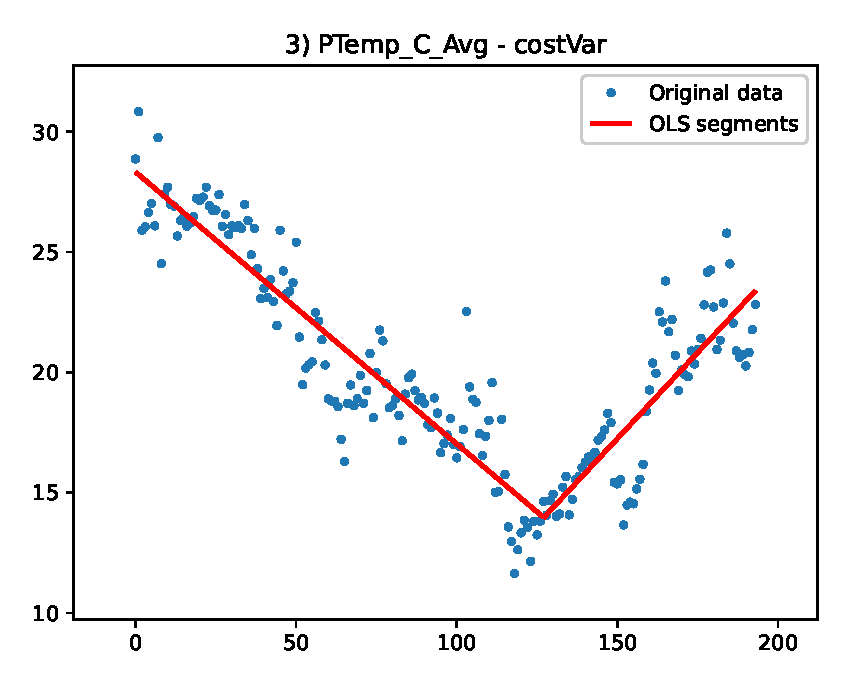
\includegraphics[width=0.45\textwidth]{PTemp_C_AvgCostVar.eps}
        \label{fig:temperature}%
        }%
    \hfill%
    \subfloat[Minimum battery current]{%
        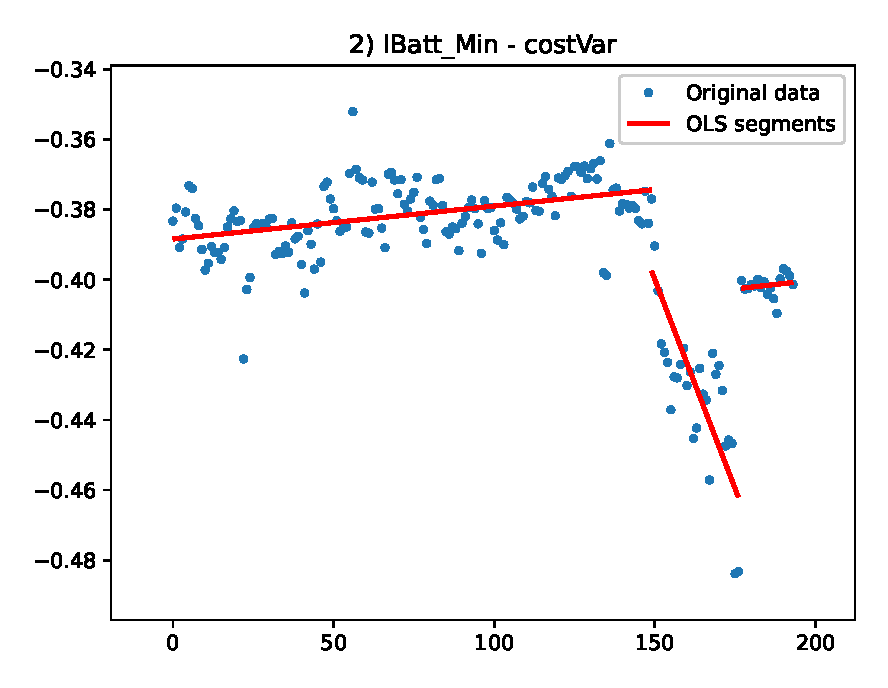
\includegraphics[width=0.45\linewidth]{IBatt_MinCostVar.eps}%
        \label{fig:battery}%
        }%
    \caption{Environmental dataseries}
    \label{fig:environ}
\end{figure*}


% Example of a figure that spans the whole page width and with subfigures. The same concept works for tables, too.
\begin{figure}[H]
	%\isPreprints{}{% This command is only used for ``preprints''.
		\begin{adjustwidth}{-\extralength}{0cm}
			\centering
			%} % If the paper is ``preprints'', please uncomment this parenthesis.
		\subfloat[\centering]{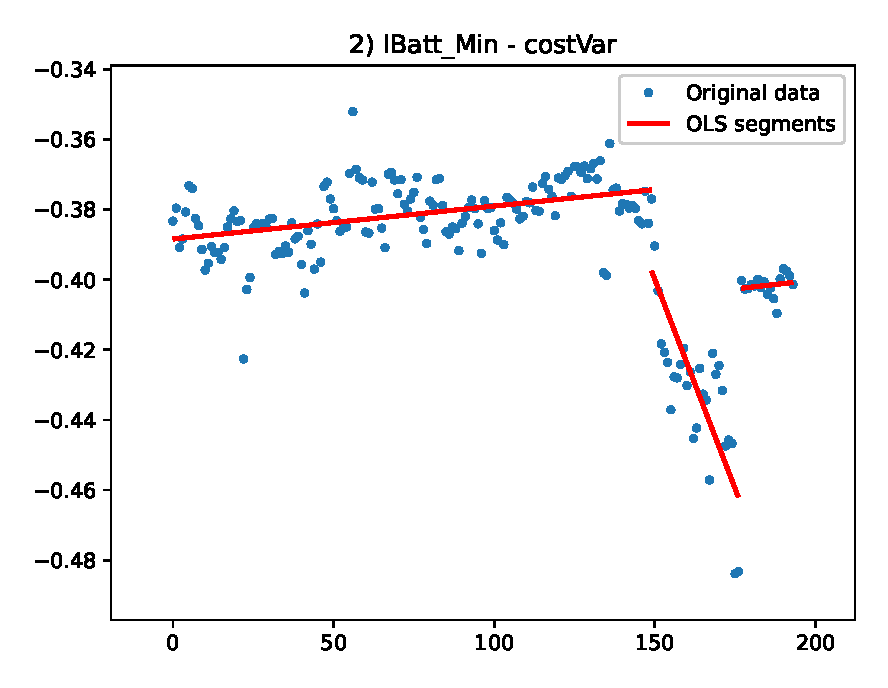
\includegraphics[width=5.0cm]{IBatt_MinCostVar.eps}}
		%\hfill
		\subfloat[\centering]{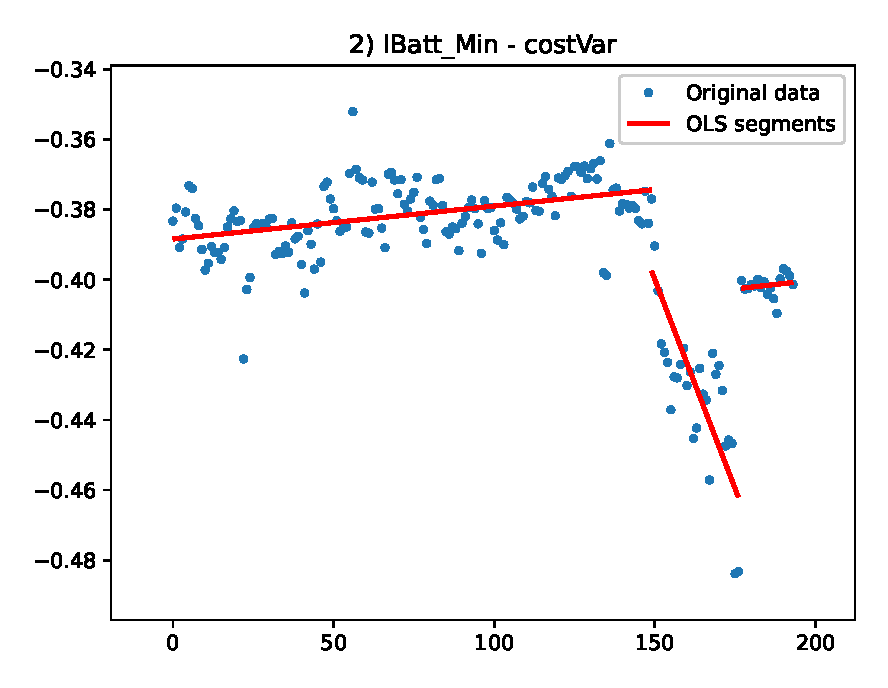
\includegraphics[width=5.0cm]{IBatt_MinCostVar.eps}}\\
		\subfloat[\centering]{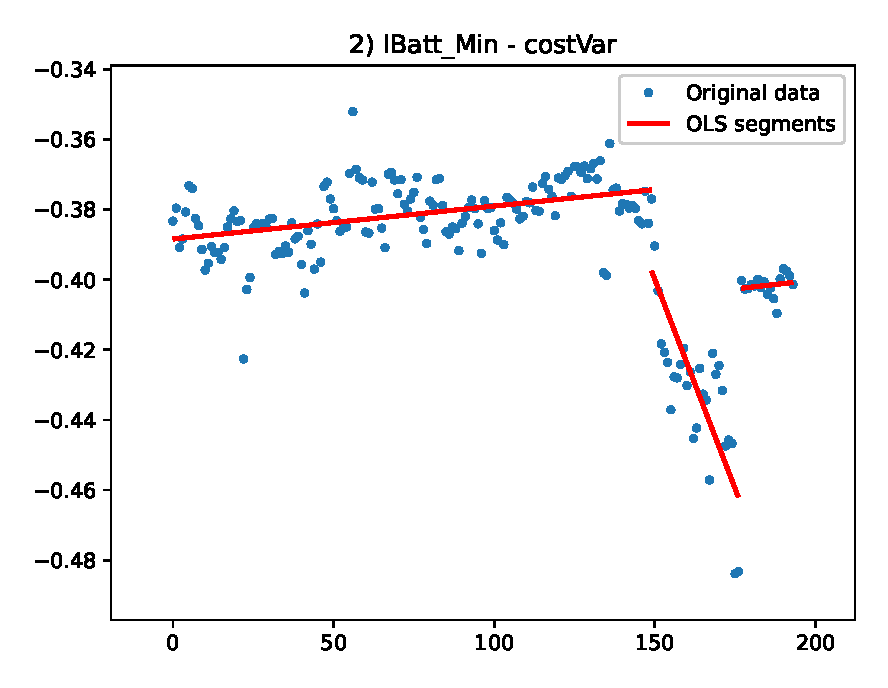
\includegraphics[width=5.0cm]{IBatt_MinCostVar.eps}}
		%\hfill
		\subfloat[\centering]{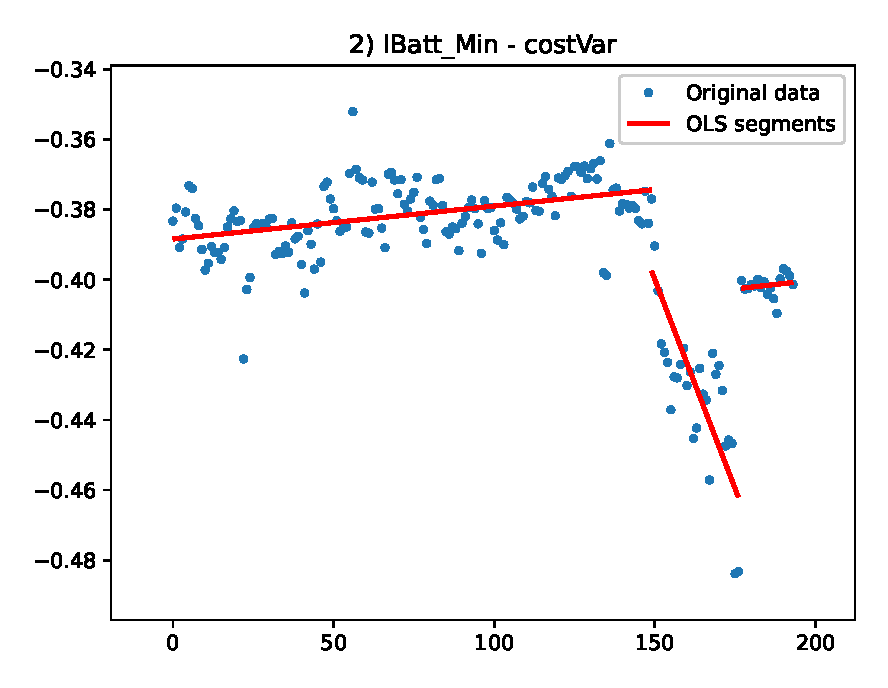
\includegraphics[width=5.0cm]{IBatt_MinCostVar.eps}}
		\end{adjustwidth}
	\caption{This is a wide figure. Schemes follow the same formatting. If there are multiple panels, they should be listed as: (\textbf{a}) Description of what is contained in the first panel. (\textbf{b}) Description of what is contained in the second panel. (\textbf{c}) Description of what is contained in the third panel. (\textbf{d}) Description of what is contained in the fourth panel. Figures should be placed in the main text near to the first time they are cited. A caption on a single line should be centered.\label{fig2}}
\end{figure} 


Not surprisingly, the set partitioning model could always produce the better solution, as it was the only algorithm that explicitly used the proposed cost function for optimization. More interesting is the limited computational time needed to solve instances with up to a few hundred variables, while the "curse of dimensionality" becomes apparent when solving instances with more than 1000 variables. The healthcare instance, here only a validation case, proves that the approach is also effective for nonlinear segmentation, but the search for optimal fitting parameters requires a very high CPU time. The figures \ref{fig:environ} show the solution for two environmental data series, while the figures \ref{fig:nonenv} show the two non environmental data series.
\vspace{-0.8cm}
\begin{figure*}[ht]
    \centering
    \subfloat[Bitcoin - USD exchange rate]{%
        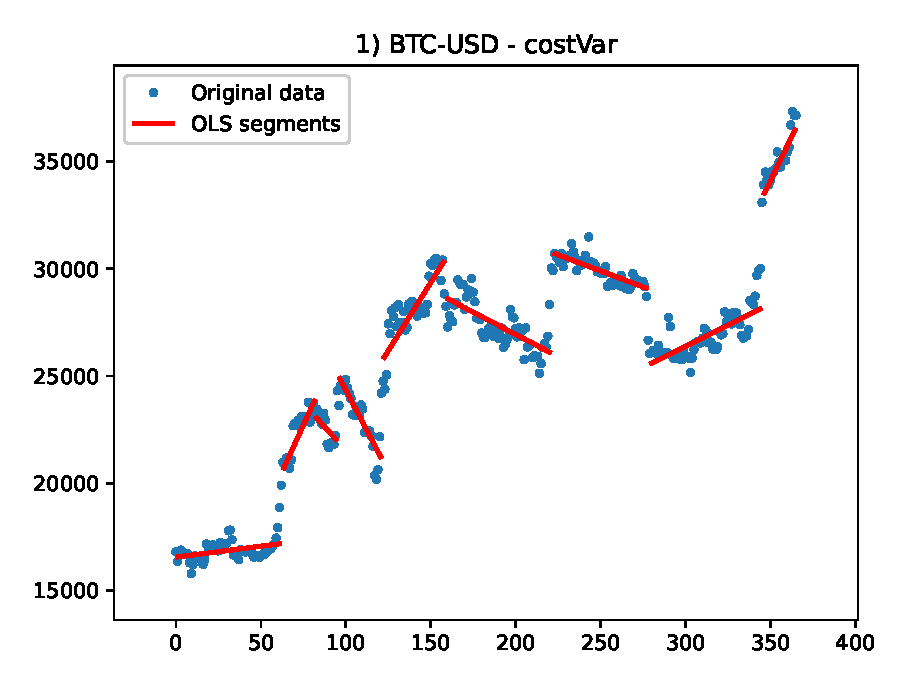
\includegraphics[width=0.45\textwidth]{BTC-USDcostVar.eps}
        \label{fig:bitcoins}%
        }%
    \hfill%
    \subfloat[Covid Italy 2022]{%
        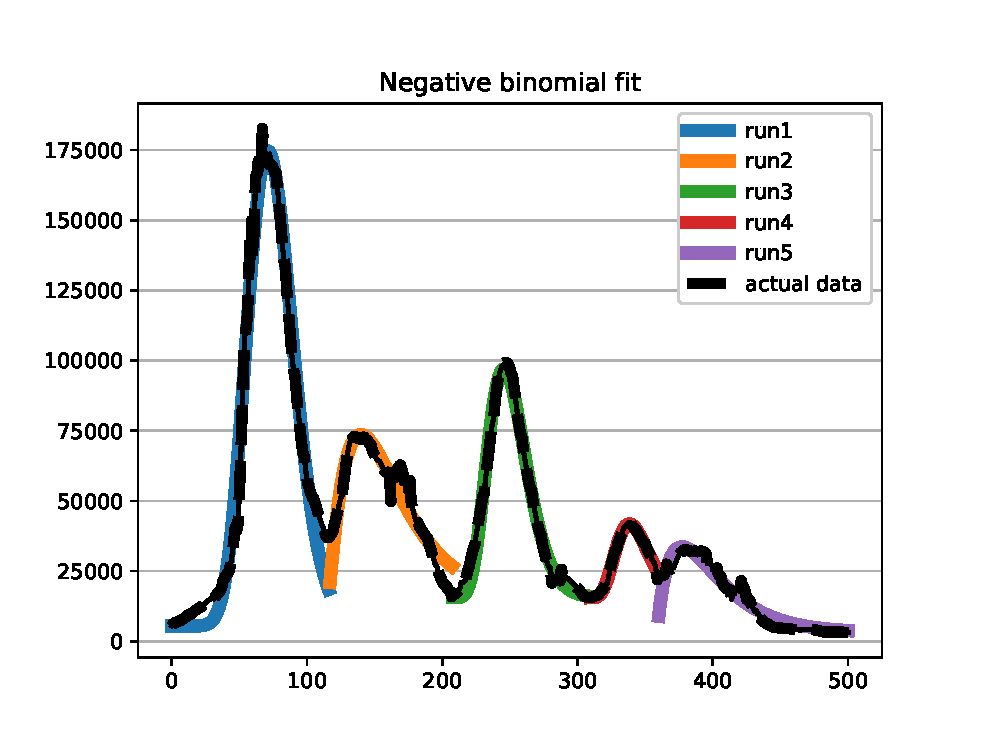
\includegraphics[width=0.45\linewidth]{negativeBinFit.eps}%
        \label{fig:covid}%
        }%
    \caption{Economics and healthcare dataseries}
    \label{fig:nonenv}
\end{figure*}

%% Example of a page in landscape format (with table and table footnote).
%\startlandscape
%\begin{table}[H] %% Table in wide page
%%\isPreprints{\centering}{} % This command is only used for ``preprints''.
%\caption{This is a very wide table.\label{tab3}}
%	\begin{tabularx}{\textwidth}{CCCC}
	%		\toprule
	%		\textbf{Title 1}	& \textbf{Title 2}	& \textbf{Title 3}	& \textbf{Title 4}\\
	%		\midrule
	%		Entry 1		& Data			& Data			& This cell has some longer content that runs over two lines.\\
	%		Entry 2		& Data			& Data			& Data\textsuperscript{1}\\
	%		\bottomrule
	%	\end{tabularx}
%%\isPreprints{}{% This command is only used for ``preprints''.
	%	\begin{adjustwidth}{+\extralength}{0cm}
		%%} % If the paper is ``preprints'', please uncomment this parenthesis.
	%		\noindent\footnotesize{\textsuperscript{1} This is a table footnote.}
	%%\isPreprints{}{% This command is only used for ``preprints''.
		%	\end{adjustwidth}
	%%} % If the paper is ``preprints'', please uncomment this parenthesis.
%\end{table}
%\finishlandscape


\section{Conclusions} \label{sec:conclusions}

The paper presents an MIP-based approach, both a Lagrangian matheuristic and an exact model, to time series segmentation. The underlying mathematical model is able to adapt to different requirements on the resulting model, making it more tolerant to residuals or more representative of short trends. 
The analysis imposes no constraints on the model associated with each segment, which can be linear, polynomial, or defined on any distribution function of interest. It can even be a combination of different models, allowing for linearity on some segments and, for example, exponential increases on others.

This flexibility comes at the cost of having to solve a NP problem on large size instances. The increase in effectiveness of general MIP solvers allows to consider the solution of real-world instances to optimality, and it also provides the basis for the design of mathematically grounded heuristics. We report preliminary results on sensor data series obtained in an environmental monitoring, but also two experiments on financial and healthcare use cases.

The results so far provide only a first indication of the possibilities offered by mathematical models, but also of the difficulties to be overcome. Besides the obvious limit imposed by the NP-hardiness of the problem (the "curse of dimensionality"), which is only partially alleviated by heuristic solving, there are problem-specific issues to be faced, such as which cost function to use or which constraint to impose on the runs. In fact, the final result is only indirectly determined by our model, and there are still cases where results are unsatisfactory to the eye, even though they are numerically satisfying. 
Current results have already proven useful in the motivating application domain, both for missing value imputation and for short-term forecasting, obtained by decomposing the series down to the last segment and using the identified components to extend it into the near future. Moreover, these results do not seem to be affected by the application domain.

%%%%%%%%%%%%%%%%%%%%%%%%%%%%%%%%%%%%%%%%%%
\vspace{6pt} 

%%%%%%%%%%%%%%%%%%%%%%%%%%%%%%%%%%%%%%%%%%
%% optional
%\supplementary{The following supporting information can be downloaded at:  \linksupplementary{s1}, Figure S1: title; Table S1: title; Video S1: title.}

% Only for journal Methods and Protocols:
% If you wish to submit a video article, please do so with any other supplementary material.
% \supplementary{The following supporting information can be downloaded at: \linksupplementary{s1}, Figure S1: title; Table S1: title; Video S1: title. A supporting video article is available at doi: link.}

% Only used for preprtints:
% \supplementary{The following supporting information can be downloaded at the website of this paper posted on \href{https://www.preprints.org/}{Preprints.org}.}

% Only for journal Hardware:
% If you wish to submit a video article, please do so with any other supplementary material.
% \supplementary{The following supporting information can be downloaded at: \linksupplementary{s1}, Figure S1: title; Table S1: title; Video S1: title.\vspace{6pt}\\
%\begin{tabularx}{\textwidth}{lll}
%\toprule
%\textbf{Name} & \textbf{Type} & \textbf{Description} \\
%\midrule
%S1 & Python script (.py) & Script of python source code used in XX \\
%S2 & Text (.txt) & Script of modelling code used to make Figure X \\
%S3 & Text (.txt) & Raw data from experiment X \\
%S4 & Video (.mp4) & Video demonstrating the hardware in use \\
%... & ... & ... \\
%\bottomrule
%\end{tabularx}
%}

%%%%%%%%%%%%%%%%%%%%%%%%%%%%%%%%%%%%%%%%%%
\authorcontributions{All authors contributed equally to all phases of the work}

\funding{``This research received no external funding''}

\informedconsent{``Not applicable''}

\dataavailability{We encourage all authors of articles published in MDPI journals to share their research data. In this section, please provide details regarding where data supporting reported results can be found, including links to publicly archived datasets analyzed or generated during the study. } 

\acknowledgments{“During the preparation of this manuscript/study, the author(s) used GenAI only for the purposes of syntax and style checking.”}

\conflictsofinterest{``The authors declare no conflicts of interest.'' } 

%%%%%%%%%%%%%%%%%%%%%%%%%%%%%%%%%%%%%%%%%%
%% Optional

%% Only for journal Encyclopedia
%\entrylink{The Link to this entry published on the encyclopedia platform.}

\abbreviations{Abbreviations}{
The following abbreviations are used in this manuscript:
\\

\noindent 
\begin{tabular}{@{}ll}
MDPI & Multidisciplinary Digital Publishing Institute\\
DOAJ & Directory of open access journals\\
TLA & Three letter acronym\\
LD & Linear dichroism
\end{tabular}
}

%%%%%%%%%%%%%%%%%%%%%%%%%%%%%%%%%%%%%%%%%%
%% Optional
\appendixtitles{no} % Leave argument "no" if all appendix headings stay EMPTY (then no dot is printed after "Appendix A"). If the appendix sections contain a heading then change the argument to "yes".

\appendixstart
\appendix
\section[\appendixname~\thesection]{}
\subsection[\appendixname~\thesubsection]{}
The appendix is an optional section that can contain details and data supplemental to the main text---for example, explanations of experimental details that would disrupt the flow of the main text but nonetheless remain crucial to understanding and reproducing the research shown; figures of replicates for experiments of which representative data are shown in the main text can be added here if brief, or as Supplementary Data. Mathematical proofs of results not central to the paper can be added as an appendix.

\begin{table}[H] 
\caption{This is a table caption.\label{tab5}}
%\newcolumntype{C}{>{\centering\arraybackslash}X}
\begin{tabularx}{\textwidth}{CCC}
\toprule
\textbf{Title 1}	& \textbf{Title 2}	& \textbf{Title 3}\\
\midrule
Entry 1		& Data			& Data\\
Entry 2		& Data			& Data\\
\bottomrule
\end{tabularx}
\end{table}

\section[\appendixname~\thesection]{}
All appendix sections must be cited in the main text. In the appendices, Figures, Tables, etc. should be labeled, starting with ``A''---e.g., Figure A1, Figure A2, etc.

%%%%%%%%%%%%%%%%%%%%%%%%%%%%%%%%%%%%%%%%%%
%\isPreprints{}{% This command is only used for ``preprints''.
\begin{adjustwidth}{-\extralength}{0cm}
%} % If the paper is ``preprints'', please uncomment this parenthesis.
%\printendnotes[custom] % Un-comment to print a list of endnotes

\reftitle{References}


% References, variant A: external bibliography
\bibliography{mathematicsMain.bib}

\PublishersNote{}
\end{adjustwidth}
\end{document}

